\chapter{Validierung}\label{sec:chapter7}

In diesem Kapitel werden die Ergbnisse des Vergleichs der ConDec - und BPMN-Modelle aus Kapitel 5 mit Hilfe einer Studie validiert. Im Rahmen der Studie ist es nur möglich die Grundsätze der \textit{Klarheit} und der \textit{Vergleichbarkeit} zu testen.

\section{Forschungsfragen}

\textbf{Forschungsfrage 1a}: 

Ist die Punktsumme bei den Verständnisfragen insgesamt bei BPMN oder bei ConDec höher?\newline



\textbf{Forschungsfrage 1b}: 

Ist die Punktsumme bei den Verständnisfragen bei den kleinen Modellen bei BPMN oder bei ConDec höher?\newline

\textbf{Forschungsfrage 1c}: 

Ist die Punktsumme bei den Verständnisfragen bei den großen Modellen bei BPMN oder bei ConDec höher? \newline

\textbf{Forschungsfrage 1d}: 

Gibt es Unterschiede im Ergebnis in Abhängigkeit des Hintergrundwissesns der Versuchsobjekte über Prozessmodellierung?  \newline

\textbf{Forschungsfrage 2a}: 

Werden bei den Meinungsfragen insgesamt die Modelle von BPMN oder von ConDec präferiert? \newline

\textbf{Forschungsfrage 2b}: 

Werden bei den Meinungsfragen bei den kleinen Modellen die von BPMN oder von ConDec präferiert?\newline

\textbf{Forschungsfrage 2c}: 

Werden bei den Meinungsfragen bei den großen Modellen die von BPMN oder von ConDec präferiert?\newline

\section{Design der Studie}

Abbildung \ref{fig:UmfrageStruktur} kann die Struktur der Umfrage entnommen werden.
Bei der Studie wurden zwei Fragebögen eingesetzt. Die 32 Teilnhemer der Studie wurden deswegen zufallsbedingt in zwei Gruppen (je 16 Personen) eingeteilt. Zunächst wurden den Probanden allgemeine demographische Fragen gestellt (Geschlecht, Alter, Hintergrundwissen zu imperativer und deklarativer Modellierung, Hintergrundwissen zu den Software Engineering Prozessmodellen Scrum, Open UP und V-Modell XT).\newline
Anschließend wurden den Teilnehmern Verständnisfragen zu ausgewählten Modellen gestellt.
Es wurden die vier  Modellpaare \textit{Lösungsinkrement entwickeln (Open UP)}, \textit{Scrum}, \textit{Systementwicklungsprojekt AG/AN} und \textit{Phasen Open UP -Inception}  aus Kapitel 5 ausgewählt. Hierbei wurde darauf geachtet, dass es sich um zwei kleine Modelle (<= 5 Aktivitäten) und zwei große Modelle (> 5 Aktivitäten) handelt. Gruppe 1 startete mit einem deklarativen Prozess und Gruppe 2 mit dem entsprechenden imperativen Prozess. Somit wurden von jeder Gruppe zwei imperative und zwei deklarative Prozesse bearbeitet.  \newline
Im letzten Teil des Fragebogens wurden den Probanden noch vier Modellpaare direkt gegenüber gestellt und sie wurden nach Ihrem präferierten Modell (deklarativ oder imperativ) gefragt und mussten in einem Freitextfeld den Grund für Ihre Entscheidung angeben. Auch hier wurden den Teilnehmern wiederum zwei kleine (<= 5 Aktivitäten) und zwei große (> 5 Aktivitäten)  Modelle gezeigt. Hier wurden die Modelle \textit{System spezifizieren (V-Modell XT)}, \textit{Phasen des Open UP}, \textit{Inkrementelle Entwicklung durchführen (V-Modell XT)} und \textit{Release deployen} ausgewählt. \newline
Die semantische Gleichheit der Modellpaare wurde wie bereits in Kapitel 5 erwähnt durch das Testen von validen Pfaden durch die jeweiligen Modelle sichergestellt.\newline

\begin{figure}[htp]
\begin{center}
  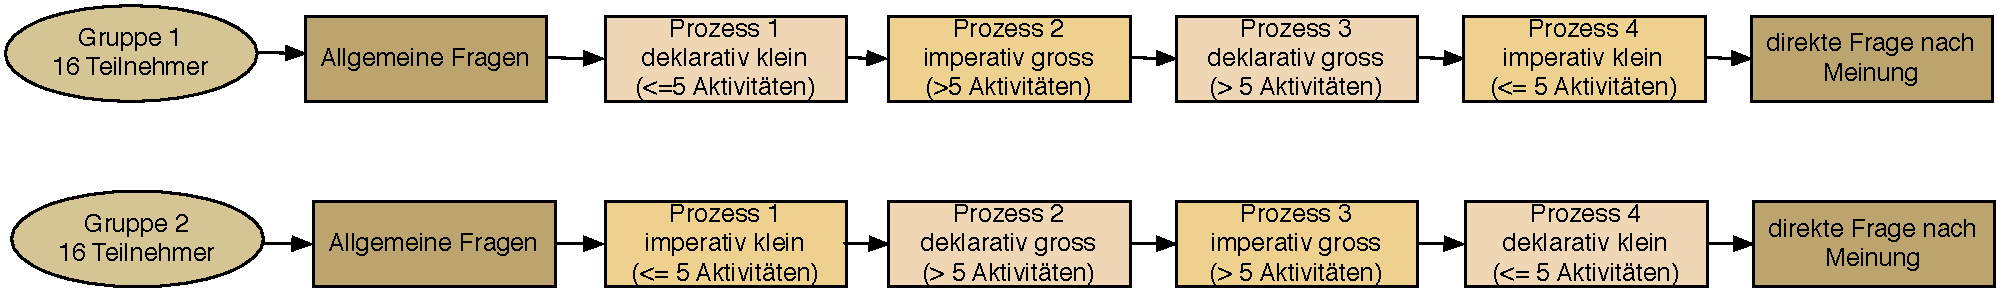
\includegraphics [width=\textwidth]{UmfrageStruktur} %pdf, jpg, png...
  \caption{Struktur der Umfrage}
  \label{fig:UmfrageStruktur}
\end{center}
\end{figure}

\subsubsection{Verständnisfragen}

Zu jedem Modell wurden den Teilnehmern jeweils acht Verständnisfragen gestellt. Diese zielten auf das Verständnis der möglichen Reihenfolge der Aktivitäten, mögliche Start- und Endaktivitäten, allgemeine informationen aus dem Modell sowie parallele Abläufe von Aktivitäten, sich ausschließende Aktivitäten und die Anzahl möglicher Ausführungen von Aktivitäten.\newline
Die Teilnehmer konnten bei der Beantwortung der Fragen zwischen vier Antwortmöglichkeiten wählen: \textit{Ja}, \textit{Nein}, \textit{Geht nicht aus Modell hervor} und \textit{Unentschlossen}.

\subsubsection{Umfragewerkzeug und Durchführung}

Zur Durchführung wurde das Fragebogenwerkzeug \textit{Limesurvey} verwendet. Der entsprechende Link zum Fragebogen sowie eine kleine Legende zur Notationsübersicht von Declare und BPMN wurde den Teilnehmern per E-Mail zugeschickt. Die entsprechenden Antworten der Probanden wurden automatich von \textit{Limesurvey} gespeichert. Weiterhin war es dort möglich die jeweilige Zeit, welche die Probanden zur Bearbeitung Verständnisfragen benötigt haben, mit zu messen. Die gespeicherten Daten können aus \textit{Limesurvey} für verschiedene exterene Anwendungen exportiert werden (z.B als Excel, CSV oder für SPSS).

\subsubsection{Auswertung}

Für jede richtige Antwort wurde ein Punkt vergeben. Für jede falsche Antwort gab es null Punkte. Auch \textit{Unentschlossen} wurde als falsche Antwort gewertet. Die einzelnen Punkte wurden dann pro Frage aufsummiert, so dass ein maximaler wert Pro Frage von 1 möglich ist.

\subsection{Durchführung der Studie}

\subsubsection{Teilnehmer}

Es wurden 32 Studenten und Doktoranden aus dem Bereich Informatik/Medieninformatik befragt. 12 Teilnehmer waren weiblich und 20 männlich (Abbildung \ref{fig:Geschlechterverteilung}). Die allgemeinen demographischen Daten der Probanden können Abbildung \ref{fig:TabelleAllgemeineDaten} entnommen werden. Diese hatten unterschiedliches Hintergrundwissen zum Thema Prozessmodellierung. Wie Abbildung \ref{fig:VerteilungImperativDeklarative} entnommen werden kann, hatten sieben Studienteilnehmer weder in imperativer noch in deklarativer Modellierung Erfahrung. 18 Probanden hatten nur in imperativer Modellierung Erfahrung, jedoch nicht in deklarativer und sieben weitere Teilnehmer hatten in beiden Modellierungssprachen Erfahrung. Die Versuchsobjekte wurden bewusst nach unterschiedlichem Hintergrundwissen zum Thema Prozessmodellierung ausgewählt, um zu prüfen, inwiefern sich die Ergebnisse bei den Verständnisfragen zwischen Personen mit viel und wenig Hintergrundwissen zum Thema Prozessmodellierung unterscheiden.\newline

\begin{figure}[htp]
\begin{center}
  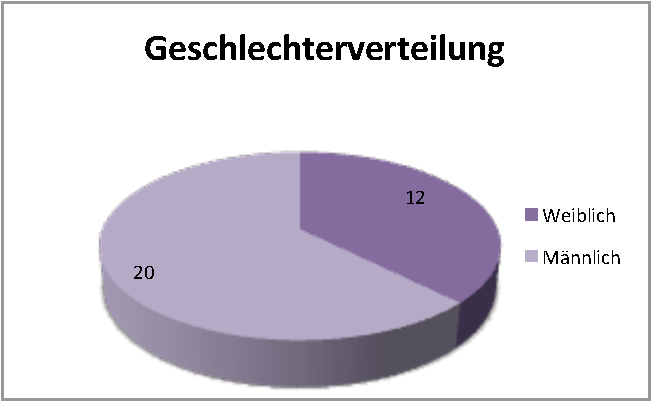
\includegraphics{Geschlechterverteilung} %pdf, jpg, png...
  \caption{Geschlechterverteilung}
  \label{fig:Geschlechterverteilung}
\end{center}
\end{figure}

\begin{figure}[htp]
\begin{center}
  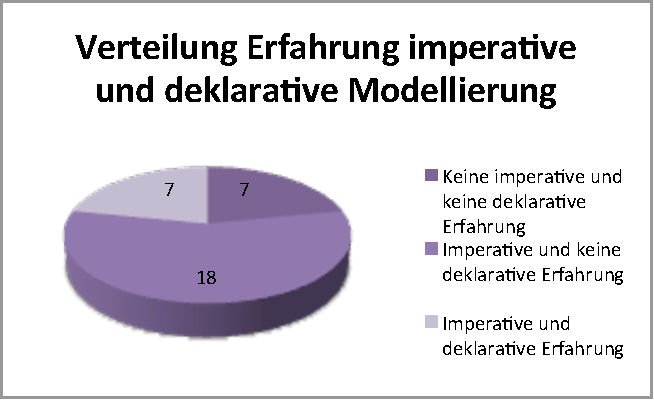
\includegraphics{VerteilungImperativDeklarative} %pdf, jpg, png...
  \caption{Verteilung Erfahrung imperative und deklarative Modellierung}
  \label{fig:VerteilungImperativDeklarative}
\end{center}
\end{figure}

\begin{figure}[htp]
\begin{center}
  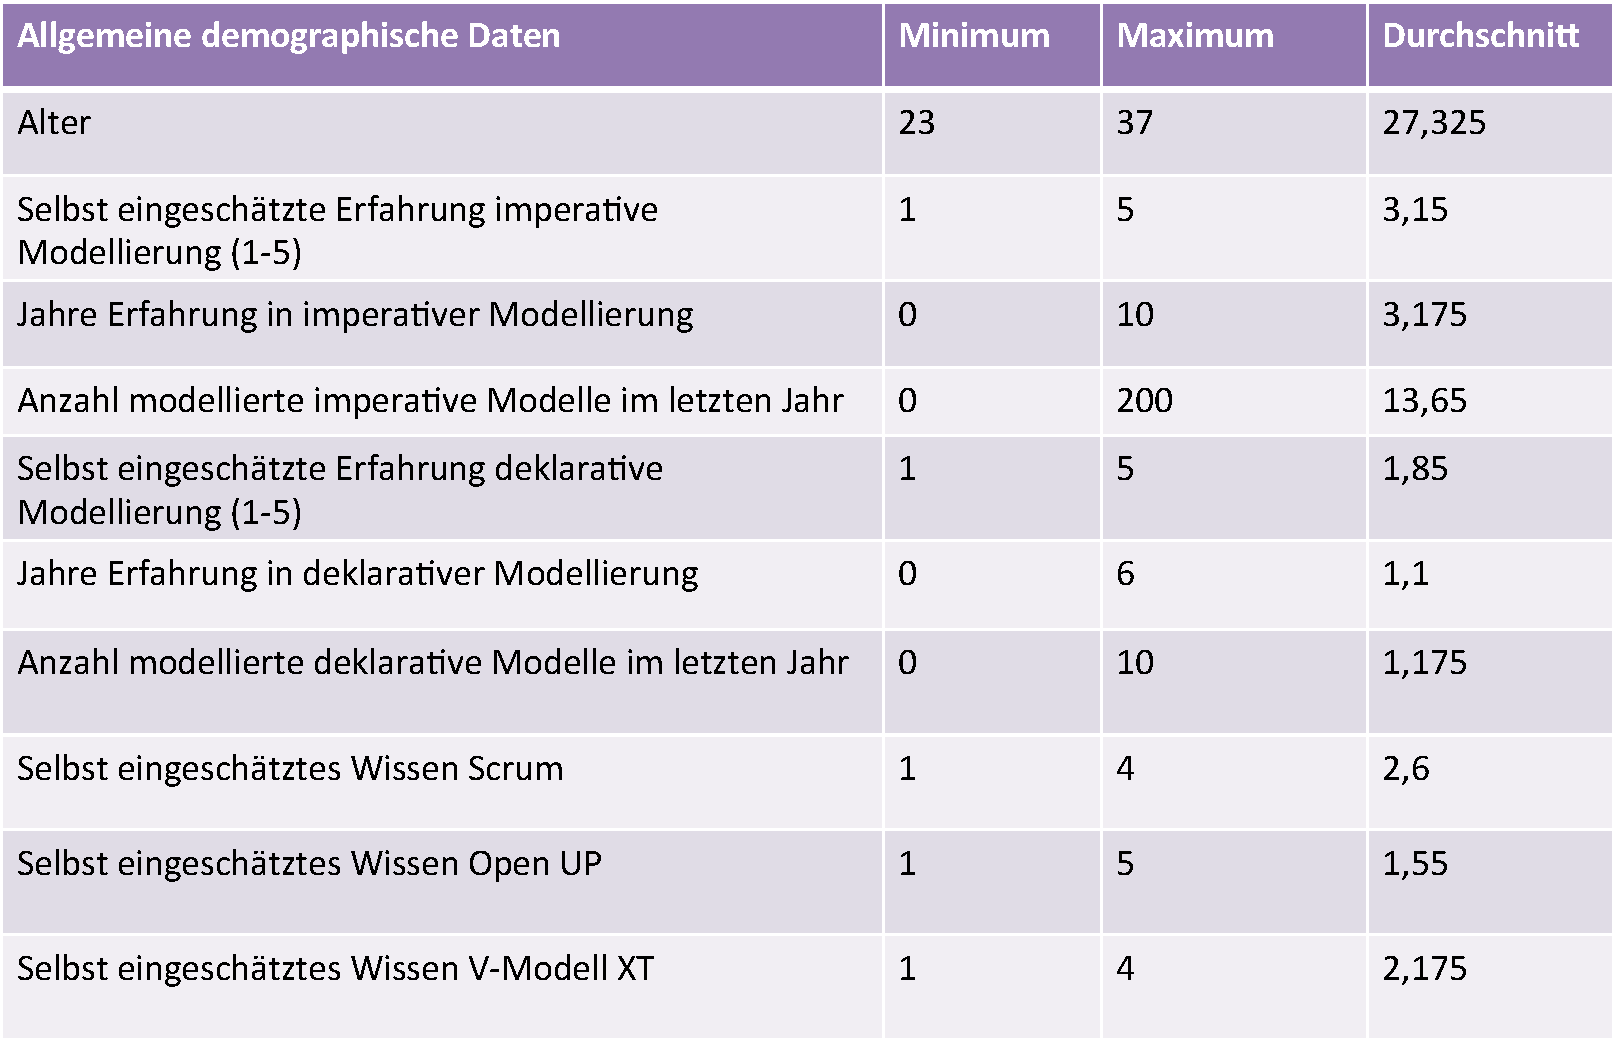
\includegraphics[width=\textwidth]{TabelleAllgemeineDaten} %pdf, jpg, png...
  \caption{Allgemeine demographische Daten}
  \label{fig:TabelleAllgemeineDaten}
\end{center}
\end{figure}



\subsubsection{Ergebnisse Verständnisfragen}

Abbildung \ref{fig:Frage1} zeigt die Ergebnisse der Verständnisfragen zum Modell \textit{Open UP: Lösungsinkrement entwickeln}. Die Ergebnisse variieren hier zwischen den deklarativen und imperativen Modellen. Während die Ergebnisse teilweise gleich sind, bzw. nur wenig voneinander abweichen, liegen die Ergebnisse der deklarativen Modelle bei den Fragen 5 und 6 deutlich unter den Ergebnissen der imperativen Modelle. \newline
Frage 5 lautete: \textit{Nach Ausführung der Aktivität \grqq Integrieren\grqq \ endet der Prozess in jedem Fall sofort}. Hier wurde von den Teilnehmern die imperative XOR- Verknüpfung besser verstanden, als die deklarative Darstellung des Ablaufes. Auch bei Frage 6 (\textit{Als erste Aktivität im Prozess kann die Aktivität \grqq Entwickeltest implementieren\grqq \ ausgeführt werden}) war den Probanden die imperative XOR-Darstellung, wohl in Verbindung mit dem BPMN Startsymbol als klaren Einstiegspunkt klarer, als die entsprechende deklarative Darstellung.\newline

\begin{figure}[htp]
\begin{center}
  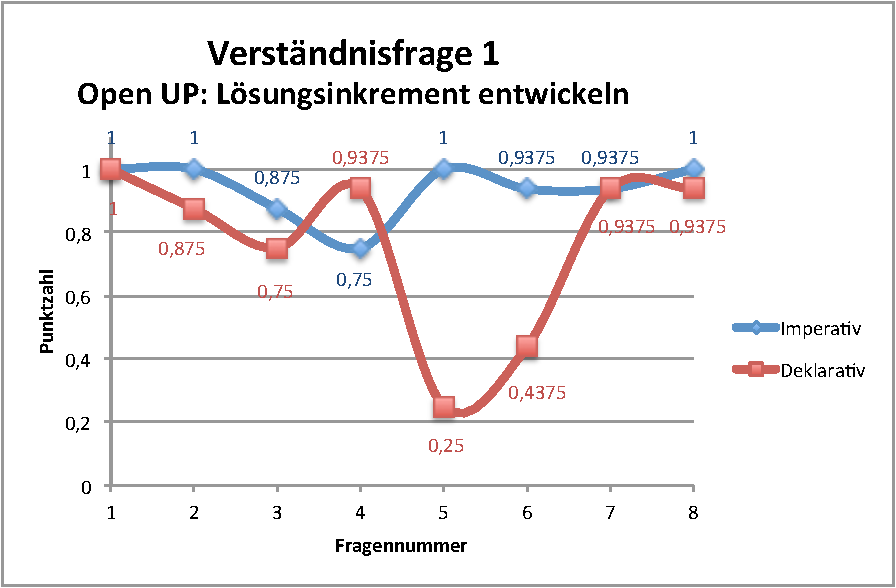
\includegraphics[scale=0.8]{Frage1} %pdf, jpg, png...
  \caption{Ergebnisse Verständnisfrage 1 aller Teilnehmer}
  \label{fig:Frage1}
\end{center}
\end{figure}


Die Ergebnisse der Verständnisfrage 2 zum Modell \textit{Scrum} von allen Teilnehmern kann Abbildung \ref{fig:Frage2} entnommen werden.  Bei Scrum handelte es sich um ein großes Modell (>5 Aktivitäten), welches sowohl viele Verzweigungen, als auch viele parallele Aktivitäten aufweist. Auch hier weichen die Ergebnisse zwischen den imperativen und deklarativen Modellen voneinander ab.\newline
Nur bei der ersten Frage (\textit{Ein Scrum Meeting dauert 15 Minuten}) schneidet der deklarative Prozess besser ab, als der imperative. Diese allgemeine Information aus dem Prozess befand sich bei beiden Prozessen in der Beschriftung der Aufgabe \textit{15-minütiges Scrum Meeting durchführen}. Der imperative Scrum-Prozess weist insgesamt mehr Elemente auf, als der deklarative. Daher fiel es wohl den Probanden hier einfacher die Übersicht über allgemeine Informationen zu behalten.\newline
Bei den Fragen 2 und 8 hat das deklarative Modell eine sehr schlechte Punktzahl erreicht. Bei Frage 2 (\textit{Die Aktivität \grqq Task abarbeiten\grqq \ kann beliebig ausgeführt werden}) konnten die Teilnehmer der XOR-Verknüpfung im imperativen Modell, welche eine Rückschleife auf die Aktivität \textit{Task abarbeiten} mehr folgen, als der Darstellung der Aktivität im deklarativen Modell. \newline
Das gleiche gilt für Frage 8 (\textit{Nach Beendigung der Aufgabe \grqq Task abarbeiten\grqq \ endet der Prozess sofort}). Auch hier wurde die Verzweigung und das damit mögliche Zurückkehren zur Aufgabe \textit{Sprint-Planning-Meeting durchführen} durch eine XOR-Verknüpfung im imperativen Modell dargestellt und war somit für die Teilnehmer klarer verständlich.\newline


\begin{figure}[htp]
\begin{center}
  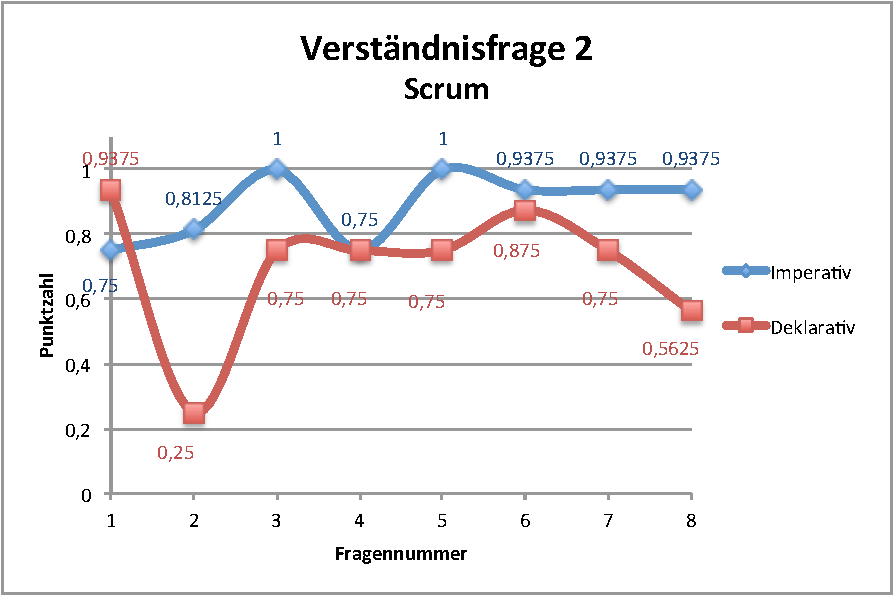
\includegraphics[scale=0.8]{Frage2} %pdf, jpg, png...
  \caption{Ergebnisse Verständnisfrage 2 aller Teilnehmer}
  \label{fig:Frage2}
\end{center}
\end{figure}

Beim Modell \textit{V-Modell: Systementwicklungsprojekt AG/AN} der Verständnisfrage 3 lagen die Ergebnisse des deklarativen Modell bis auf Frage 3 immer unter denen des imperativen Modells. Starke Abweichung gab es bei den Fragen 2, 4, 5, 7. \newline
Bei Frage 2 (\textit{Die Aktivitäten \grqq Prototypische Entwicklung durchführen\grqq, \grqq Komponentenbasierte Entwicklung durchführen\grqq \ und \grqq Inkrementelle Entwicklung durchführen\grqq \ können parallel zueinander ausgeführt werden}) war den Teilnehmern, welche das deklarative Modell bearbeiten mussten, die Notation des Constraints \textit {Exclusive Choice 1 of 3} nicht ganz klar. Sechs der 16 Probanden kreuzten hier entweder \textit{Ja} oder \textit{Unentschlossen} an.\newline
Sowohl Frage 4 (\textit{Nach Ausführung der Aktivität \grqq System abnehmen\grqq \ kann die Aktivität \grqq Anforderungen festlegen\grqq \ ausgeführt werden}, als auch Frage 5 (\textit{Nach Ausführung der Aktivität \grqq System abnehmen\grqq \ kann die Aktivität \grqq Projekt ausschreiben\grqq \ ausgeführt werden}) zielten wieder auf Verzweigungen des Prozesses ab und waren den Teilnehmern mit dem imperativen Prozess klarer. \newline
Frage 7 (\textit{Nach Ausführung der Aktivität \grqq Projekt abschließen\grqq \ endet der Prozess}) wurde von den Probanden, welchen das imperative Modell gezeigt wurde richtiger beantwortet. Hier war im imperativen Modell durch das BPMN-Ende-Symbol den Teilnehmern das Ende des Prozesses wohl klarer, als die Darstellung durch das Constraint \textit{not succession} im deklarativen Modell.\newline

\begin{figure}[htp]
\begin{center}
  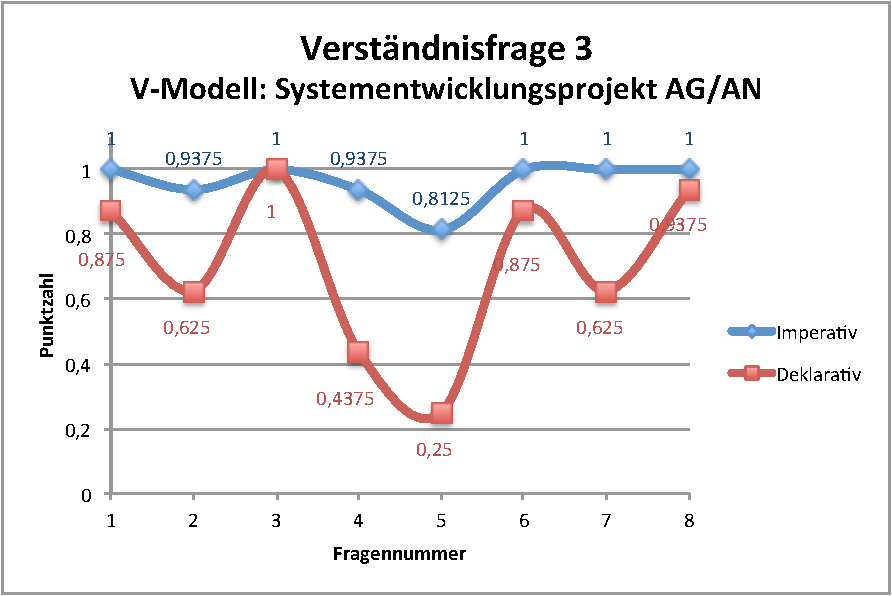
\includegraphics[scale=0.8]{Frage3} %pdf, jpg, png...
  \caption{Ergebnisse Verständnisfrage 3 aller Teilnehmer}
  \label{fig:Frage3}
\end{center}
\end{figure}

Die Ergebnisse des Prozesses \textit{Open UP: Inception} weichen zwischen den deklarativen und imperativen Modellen nicht stark voneinander ab. \newline
Lediglich bei Frage 6 (\textit{Die Aktivität \grqq Iteration planen und managen\grqq \ kann beliebig oft ausgeführt werden}) und Frage 7 (\textit{Die Aktivitäten \grqq Anforderungen identifizieren und verfeinern\grqq \ und \grqq auf technisches Vorgehen einigen\grqq \ können beliebig oft ausgeführt werden}) war den Teilnehmern wohl teilweise die funktion des Existenz (1) Constraints nicht ganz klar oder wurde übersehen.\newline

\begin{figure}[htp]
\begin{center}
  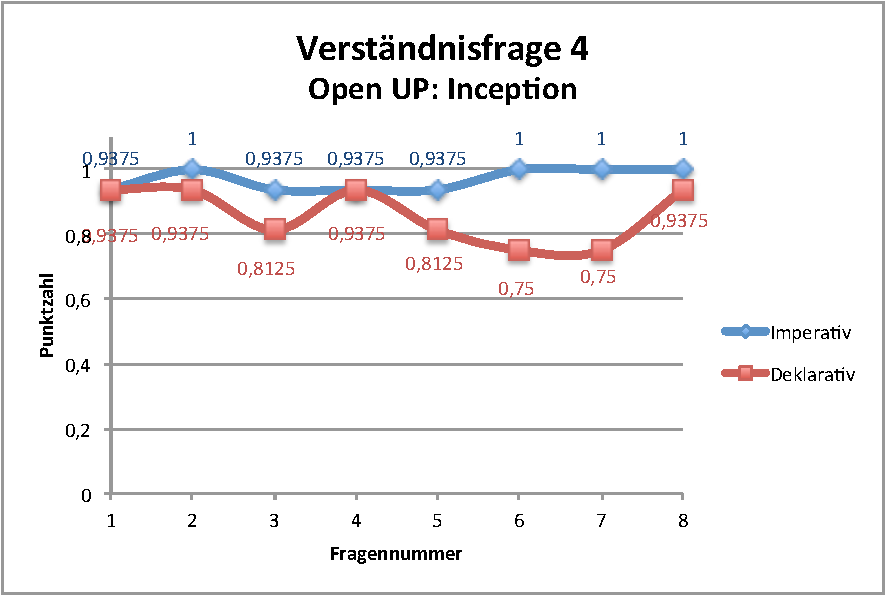
\includegraphics[scale=0.8]{Frage4} %pdf, jpg, png...
  \caption{Ergebnisse Verständnisfrage 4 aller Teilnehmer}
  \label{fig:Frage4}
\end{center}
\end{figure}

\clearpage


\subsubsection{Ergebnisse Meinungsfragen}

Abbildung \ref{fig:Meinungsfrage1} zeigt, dass 31 der 32 Befragten beim Modell \textit{System spezifizieren} das imperative Modell bevorzugen. Nur eine Person zog das deklarative Modell vor. Hierbei handelt es sich um einen Teilnehmer, welcher weder in imperativer, noch in deklarativer Prozessmodellierung Erfahrung aufweist. Als Begründung für den Vorzug des deklarativen Modells gab der Befragte an, das Modell sei kompakter, jedoch sei auch mehr Verständnis notwendig.\newline
Die Probanden, welche das imperative Modell bevorzugten gaben verschiedene Gründe hierfür an. Unter anderem nannten sie als Grund die klarere Struktur des BPMN-Modells, die vielen unterschiedlichen/komplexen Elemente im deklarativen Modell oder auch die klare Rollenverteilung durch die Swimlanes. Einige Befragte gaben auch ihre bessere Kenntniss in imperativen Prozessmodellierungssprachen als Grund an.\newline

\begin{figure}[htp]
\begin{center}
  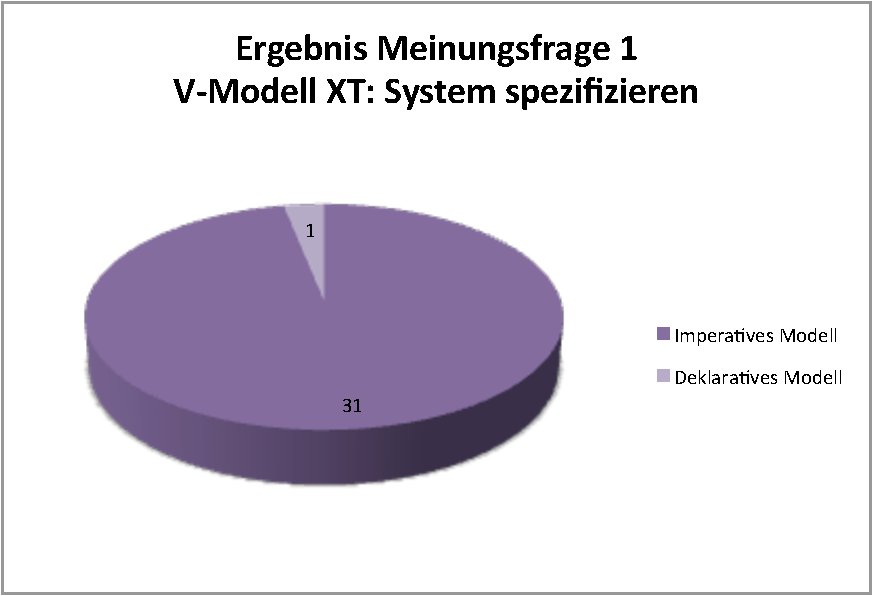
\includegraphics[scale=0.8]{Meinungsfrage1} %pdf, jpg, png...
  \caption{Ergebnisse Meinungsfrage 1 aller Teilnehmer}
  \label{fig:Meinungsfrage1}
\end{center}
\end{figure}

Ebenfalls beim Modell \textit{Phasen Open UP} bevorzugt eine deutliche Mehrheit (26 von 32 Befragten) das imperative Modell, wie Abbildung \ref{fig:Meinungsfrage2} entnommen werden kann. \newline
Hierbei verfügte nur einer der sechs Personen, welche das deklarative Modell bevorzugte auch über Erfahrung in deklarativer Modellierung. Die anderen Probanden verfügten entweder über keine Erfahrungen in beiden Modellierungssprachen (zwei) oder nur über Erfahrungen in imperativer Modellierung (drei). Als Grund für ihre Wahl gaben die Probanden beispielsweise an, dass das deklarative Modell kompakter sei und dass es klarer sei, dass nur bei Erfolg die nächste Aktivität ausgeführt wird.\newline
Die Personen, welche das imperative Modell präferierten gaben an, dass sie den Ablauf mit den Schleifen im imperativen Modell klarer finden und dass sie dem Sequenzfluss besser folgen könnten.\newline


\begin{figure}[htp]
\begin{center}
  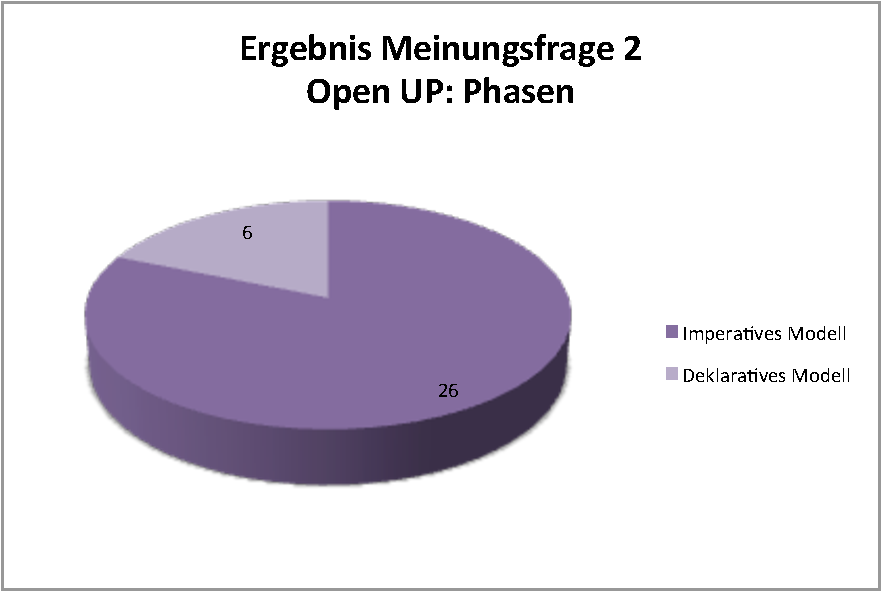
\includegraphics[scale=0.8]{Meinungsfrage2} %pdf, jpg, png...
  \caption{Ergebnisse Meinungsfrage 2 aller Teilnehmer}
  \label{fig:Meinungsfrage2}
\end{center}
\end{figure}

Die Ergebnisse des dritten Modellpaares \textit{Inkrementelle Entwicklung} zeigt Abbildung \ref{fig:Meinungsfrage3}. Demanch präferierten nur zwei Personen (eine Person mit Erfahrung sowohl in imperativer, als auch in deklarativer Modellierung, eine Person ohne imperative und deklarative Modellierungserfahrung) das deklarative Modell und 30 Probanden ziehen das imperative Modell vor.\newline
Als Grund für den Vorzug des imperativen Modells wurde die Menge an unterschiedlichen Symbolen beim imperativen Modell genannt. \newline
Die 30 Personen, welchen das imperative Modell besser gefiel gaben an, dass sie die imperative Notation verständlicher finden, der Ablauf im imperativen Modell klarer erkennbar sei, sie keinen Anhaltspunkt haben, wo im deklarativen Modell gestartet bzw. geendet wird und die vielen verschiedenen Constraints im deklarativen Modell es erschweren den Ablauf nachzuvollziehen.\newline

\begin{figure}[htp]
\begin{center}
  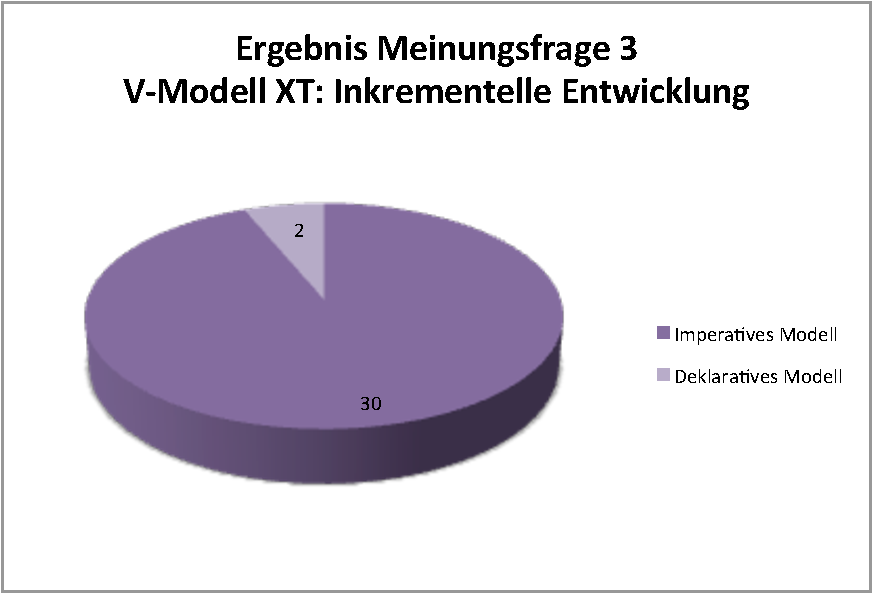
\includegraphics[scale=0.8]{Meinungsfrage3} %pdf, jpg, png...
  \caption{Ergebnisse Meinungsfrage 3 aller Teilnehmer}
  \label{fig:Meinungsfrage3}
\end{center}
\end{figure}

Beim Modell \textit{Open UP: Release deployen} präferierten neun Personen das deklarative Modell und 23 Teilnehmer das imperative Modell. Von den neun Teilnehmern, welche das deklarative Modell präferierten hatte nur einer Erfahrung in deklarativer Modellierung, einer hatte weder in deklarativer noch in imperativer Modellierung Erfahrung und sieben hatten nur in imperativer Modellierung Erfahrung. \newline
Als Begründung für die Wahl des deklarativen Modelles wurde die Übersichtlichkeit desselbigen genannt und zwar auf Grund der fehlenden Artefakte im Modell. Es wurde bemängelt, die vielen Artefakte würden das imperative Modell unübersichtlich machen.\newline
Die Probanden, welche das imperative Modell besser fanden gaben als Gründe den klaren Anfang und das klare Ende des Prozesses an, die bessere Verständlichkeit der Optionalität der Aktivität \textit{Backoutplan ausführen} und die fehlenden Artefakte im deklarativen Modell. \newline



\begin{figure}[htp]
\begin{center}
  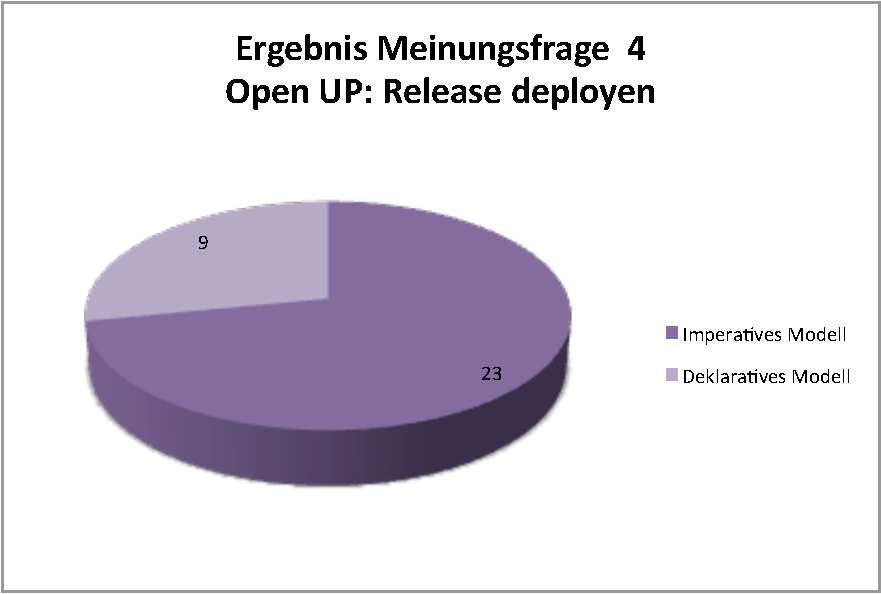
\includegraphics[scale=0.8]{Meinungsfrage4} %pdf, jpg, png...
  \caption{Ergebnisse Meinungsfrage 4 aller Teilnehmer}
  \label{fig:Meinungsfrage4}
\end{center}
\end{figure}

\clearpage

\subsection{Fazit der Studie}

Durch die Studie konnten die Ergebnisse des Vergleichs aus Kapitel 5 größtenteils belegt werden.\newline
Bei Modellen, welche viele Verzweigungen/Schleife beinhalten war für die Teilnehmer BPMN verständlicher. Dies zeigte sich beim kleinen Prozess \textit{Open UP: Lösungsinkrement entwickeln} und noch deutlicher beim großen Modell \textit{V-Modell: Systementwicklungsprojekt AG/AN}. Bei diesen beiden Prozessen sind in ConDec deutlich mehr Constraints, vor allem viele verschiedene Constraints zur korrekten Darstellung des Ablaufs notwendig, als Gateways in BPMN. Dadurch haben die ConDec-Modelle eine deutlich höhere Komplexität, als die BPMN-Modelle.\newline
Hier fällt besonders auf, dass Fragen bezüglich der Reihenfolge der Aktivitäten bei ConDec bei direkt aufeinander folgenden Aktivitäten größtenteils richtig beantwortet wurden. Jedoch bei Abläufen, bei denen es durch Verzweigungen im Prozessablauf zu einem Sprung kommt, wurden nur die Fragen zu den BPMN-Modellen größtenteils richtig beantwortet. Bei ConDec wurden diese Fragen häufig falsch beantwortet.
 







